\begin{figure}[htbp]
\centering
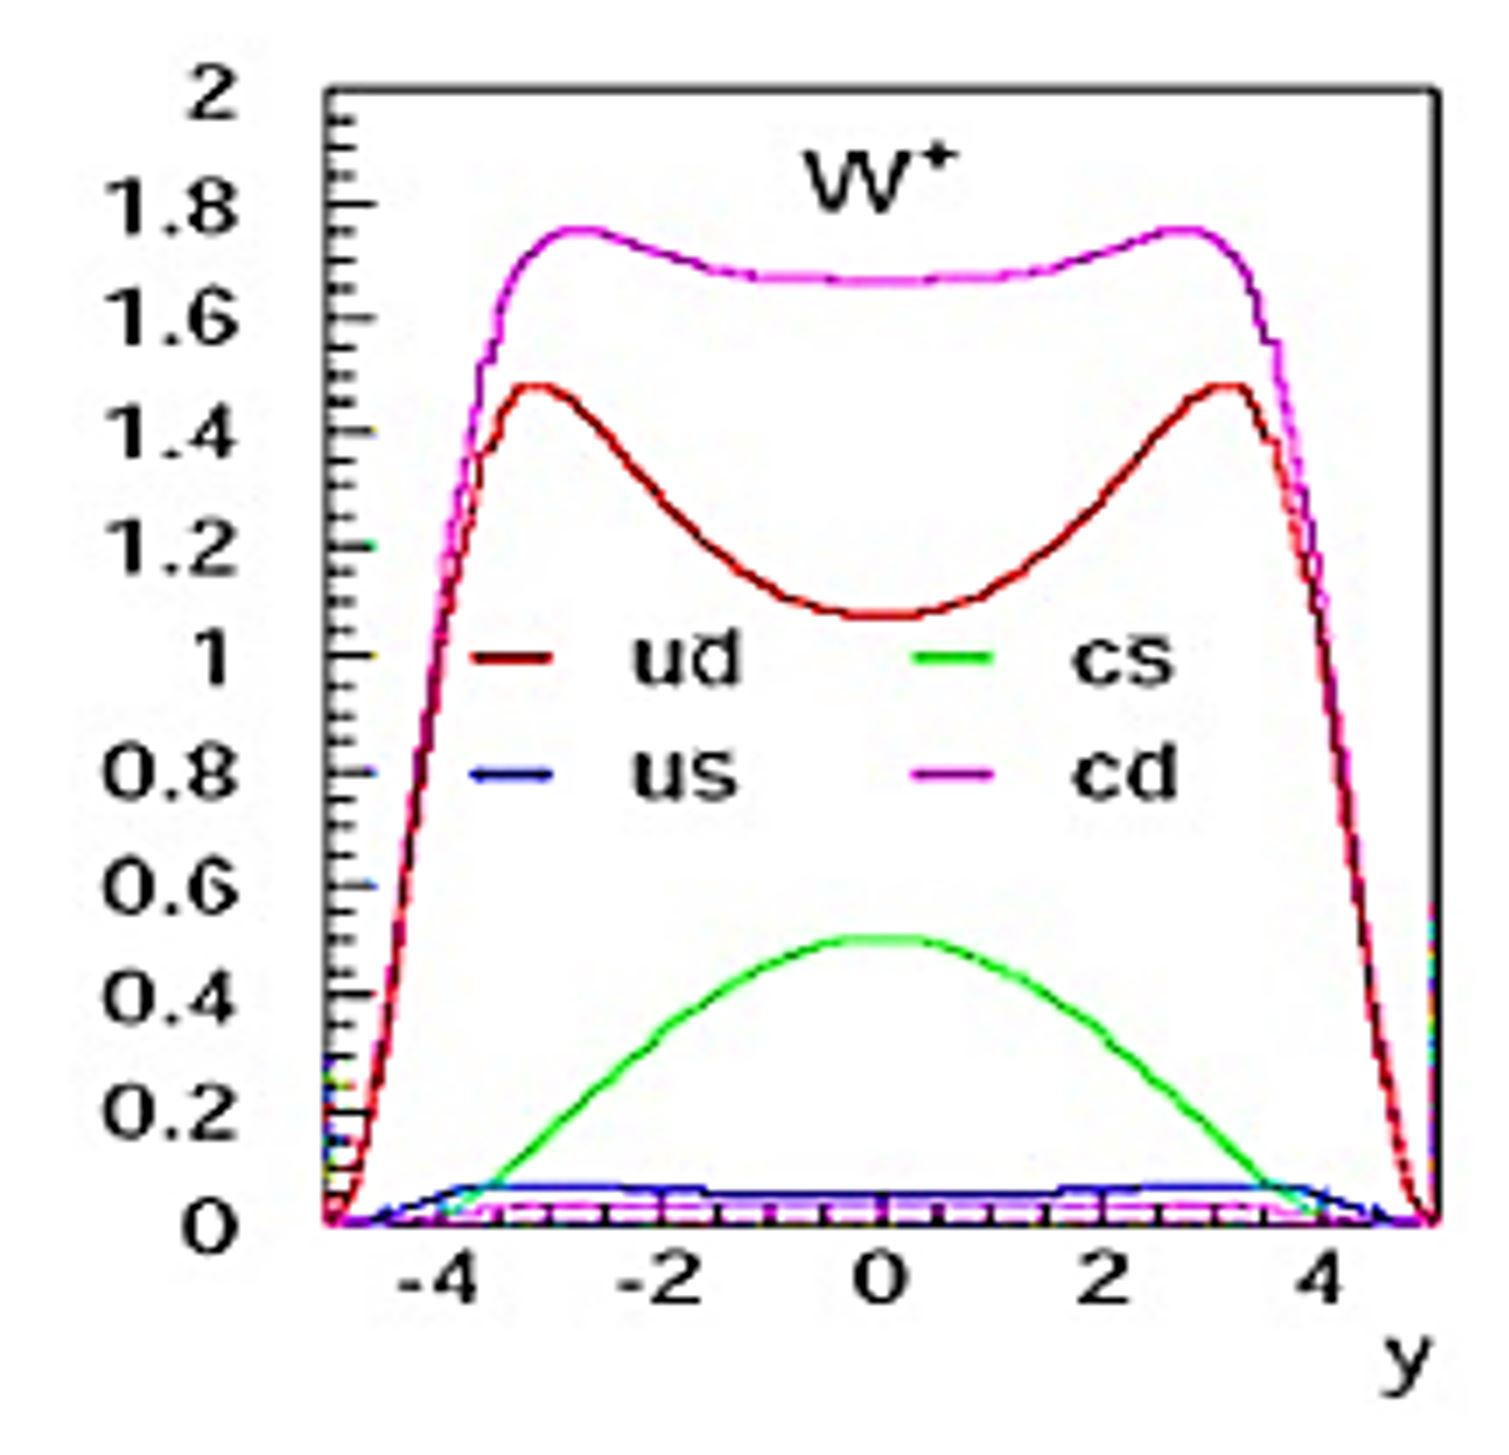
\includegraphics[width=0.31\textwidth]{plots/SM/rapidity_Wp.JPG}
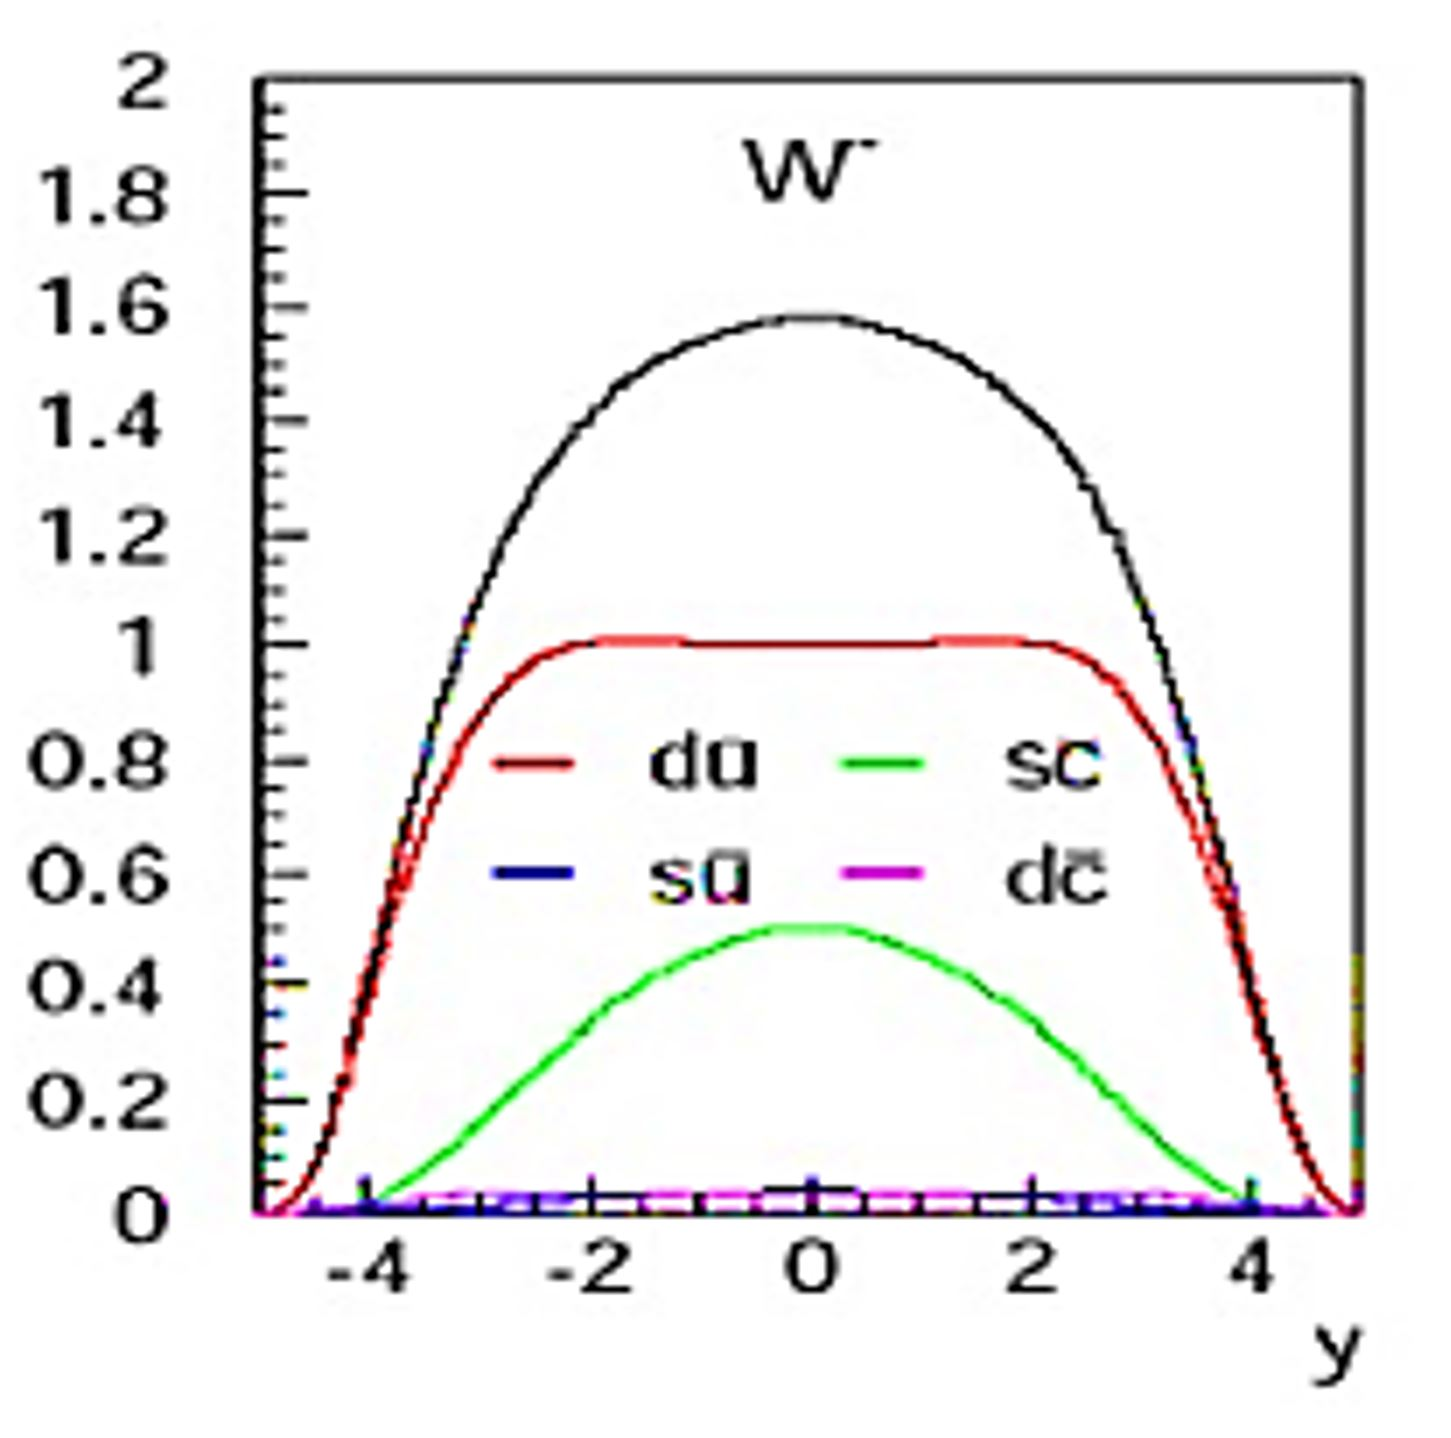
\includegraphics[width=0.30\textwidth]{plots/SM/rapidity_Wm.JPG}
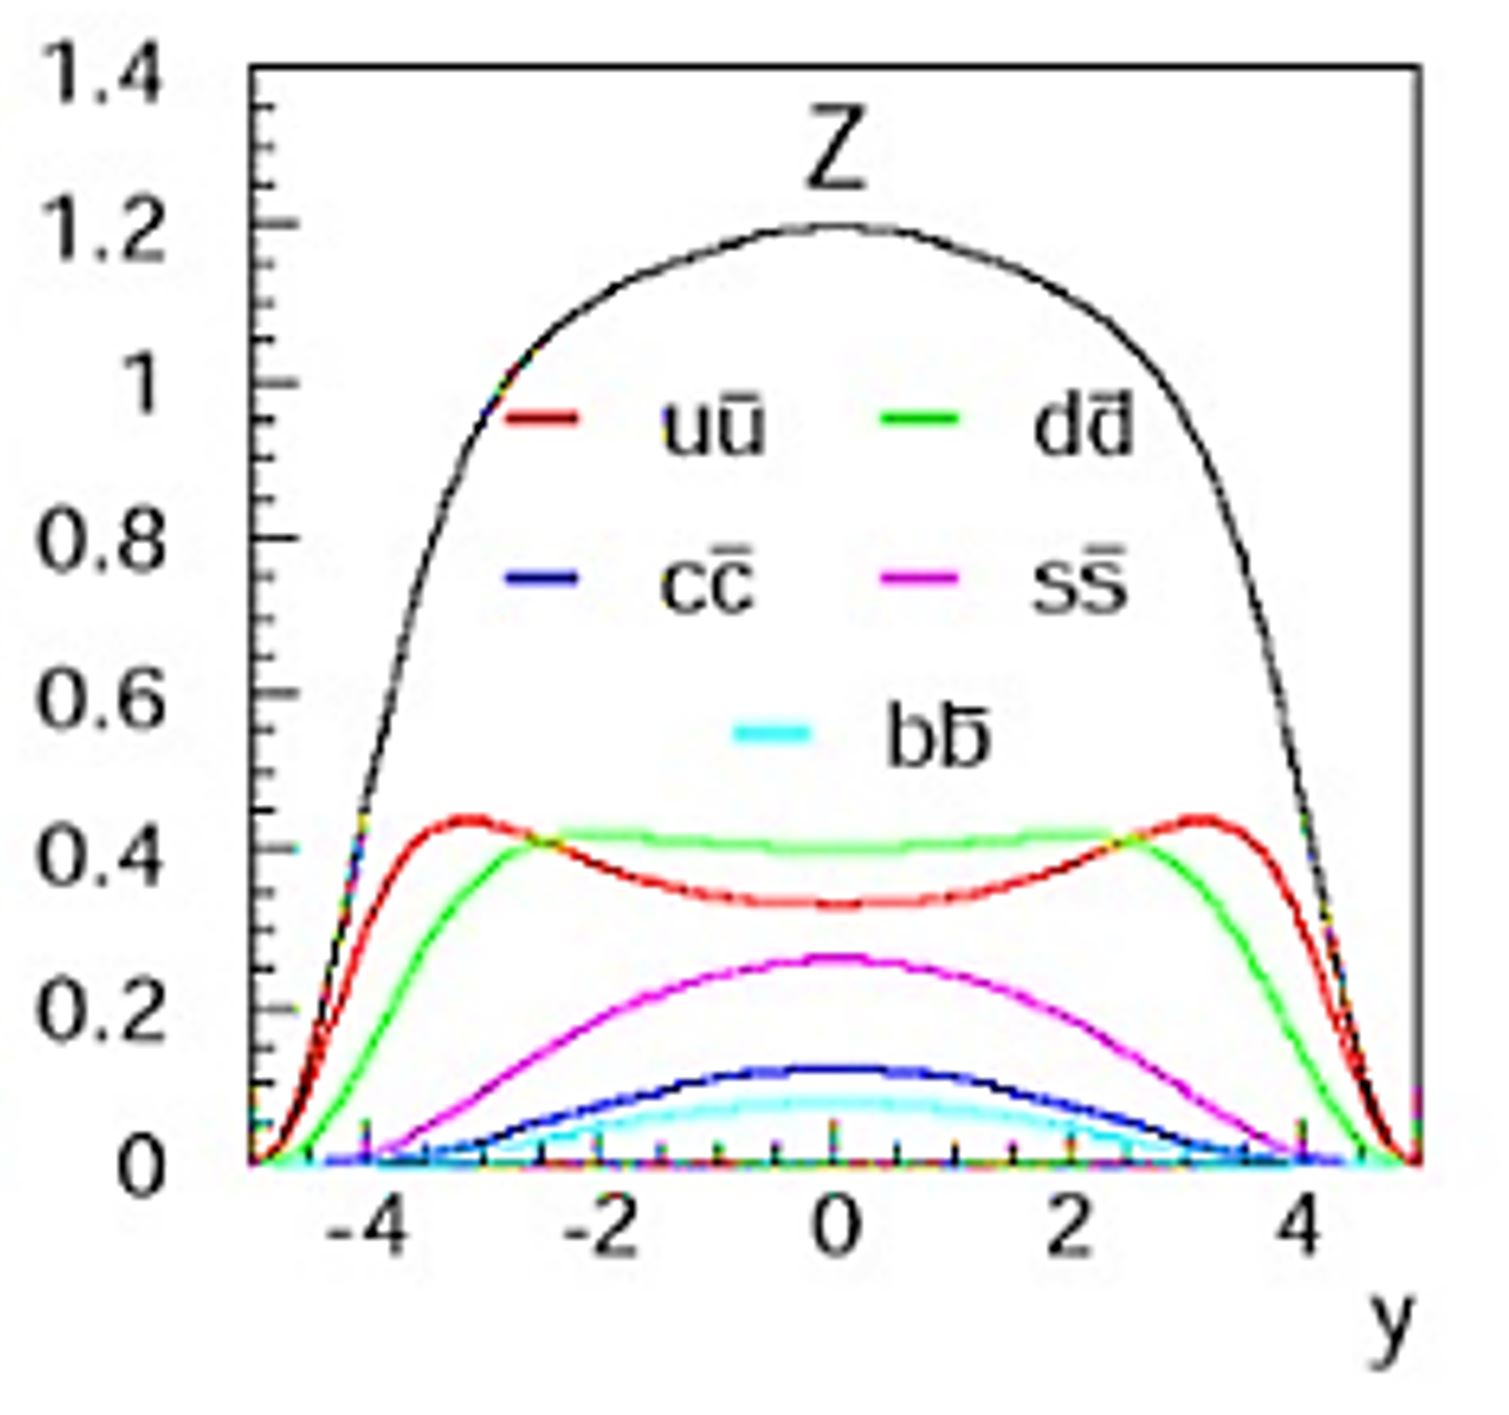
\includegraphics[width=0.32\textwidth]{plots/SM/rapidity_Z.JPG}
\caption{[Trying to make a new version from webplotdigitizer because these are ugly] Contribution of different quark flavors to the \Wp, \Wm, and \Z boson production over a range of boson rapidities. \Wp (\Wm) boson production is predominantly $u\bar{d}$ ($\bar{u}d$), while \Z boson production includes larger contributions from heavier flavors.}
\label{fig:wz_rapidity}
\end{figure}